\documentclass{article}
\usepackage[utf8]{inputenc}
\usepackage{float}
\usepackage{amsmath}
\usepackage{amssymb}
\usepackage{physics}
\usepackage{bm}
\usepackage{graphicx}

\author{Kandidatnummer: 15010}
\title{FYS3410 - Module III}
\date{April 28, 2018}

\begin{document}
\maketitle

\section*{2. FEFG and }
\emph{Introduce periodic (Born-von Karman) boundary conditions and derive the density of states (DOS) for FEFG in a finite 3D sample. Calculate values of $\varepsilon_F$, $k_F$, $v_F$ and $T_F$, i.e. Fermi energy, wavevector, velocity and temperature, respectively, for alkali metals. Explain the trend.}\\

A FEFG in 3D can at first approximation be described by the free particle Schrödinger equation in three dimensions
\begin{equation}
	-\frac{\hbar^2}{2m} \nabla^2 \bm{\psi_k}(r) = \epsilon_{\bm{k}}\bm{\psi_k}(\bm{r})
	\label{SE}
\end{equation}

Confining the electrons to a cube whose sides have length $L$ we get the following solution for the wavefunctions
\begin{equation}
	\bm{\psi}_n(\bm{r}) = A\sin(\pi n_xx/L)\sin(\pi n_yy/L)\sin(\pi n_zz/L), \quad n_x,n_y,n_z \in \mathbb{Z}
\end{equation}

Next we want to apply Born-von Karman boundary conditions. The Born-von Karman boundary condition can be represented mathematically as certain restrictions on the wavefunction in a crystal under the assumption that the wavefunction is periodic. The condition can be stated as
	\begin{equation}
		\bm{\psi}(x+L,y,z)=\bm{\psi}(x,y,z)
		\label{condition} 
	\end{equation}
For the $x$-direction and similarly for $y$ and $z$.

This is a classical particle in box problem that we know from quantum mechanics. The boundary conditions gives us the familiar solution of
\begin{equation}
	\bm{\psi_k}(\bm{r})e^{i\bm{k}\cdot\bm{r}}
	\label{pwave}
\end{equation}
With the special requirement that the wavevectors are on the form
$$ \bm{k}_x = \frac{2n_x\pi}{L} $$

It is easily shown that this satisfies equation \eqref{condition}
\begin{align*}
	\exp(i\bm{k}\cdot\bm{r}) = \exp(i\bm{k}\cdot(\bm{r}+L\bm{e}_x))\\
	\exp(i\bm{k}\cdot\bm{r}) = \exp(i\bm{k}\cdot\bm{r}) \cdot \exp(iL\bm k_x)\\
	\exp(iL\bm k_x) = 1 \implies Lk_x = 2n_x\pi
\end{align*}

Substituting equation \eqref{pwave} into \eqref{SE} we get an expression for the energies related to each wavevector

\begin{equation}
	\epsilon_{\bm{k}} = \frac{\hbar^2}{2m}\bm{k}^2 = \frac{\hbar^2}{2m}(k_x^2+k_y^2+k_z^2)
\end{equation}

Since energy and wavevector are related in this way, the energy of the possible states in k-space increase radially from the zero-vector in k-space. In the ground state of a system of N free electrons we therefore expect the occupied states to be distributed in a sphere in k-space so as to minimze the energy. The magnitude of the radius is $k_F$ and the related energy is called the Fermi energy

\begin{equation}
	\epsilon_F = \frac{\hbar^2}{2m}k_F^2
\end{equation}

We can now derive an equation for the number of different orbitals, making sure to account for the two possible electrons in each state. We divide the volume of the sphere with the volume that a each state occupies in k-space (inverse distribution density)

\begin{align}
	2*\frac{ 4\pi k_F/3 }{(2\pi/L)^3} = \frac{V}{3\pi^2}k_F^3 = N\\
	N = \frac{V}{3\pi^2}\qty(\frac{2m\epsilon}{\hbar^2})^{3/2}
\end{align}

Finally we now have what we need to find the density of states

\begin{equation}
	D(\epsilon) \equiv \dv{N}{\epsilon} = \frac{V}{2\pi^2}\qty(\frac{2m}{\hbar^2})^{3/2}\sqrt{\epsilon}
\end{equation}

\newpage
Using these relations we can calculate different values for different elements. In the figure are shown for the alkali metals Li, Na, K, Rb and Cs (in order). 

\begin{figure}[H]
	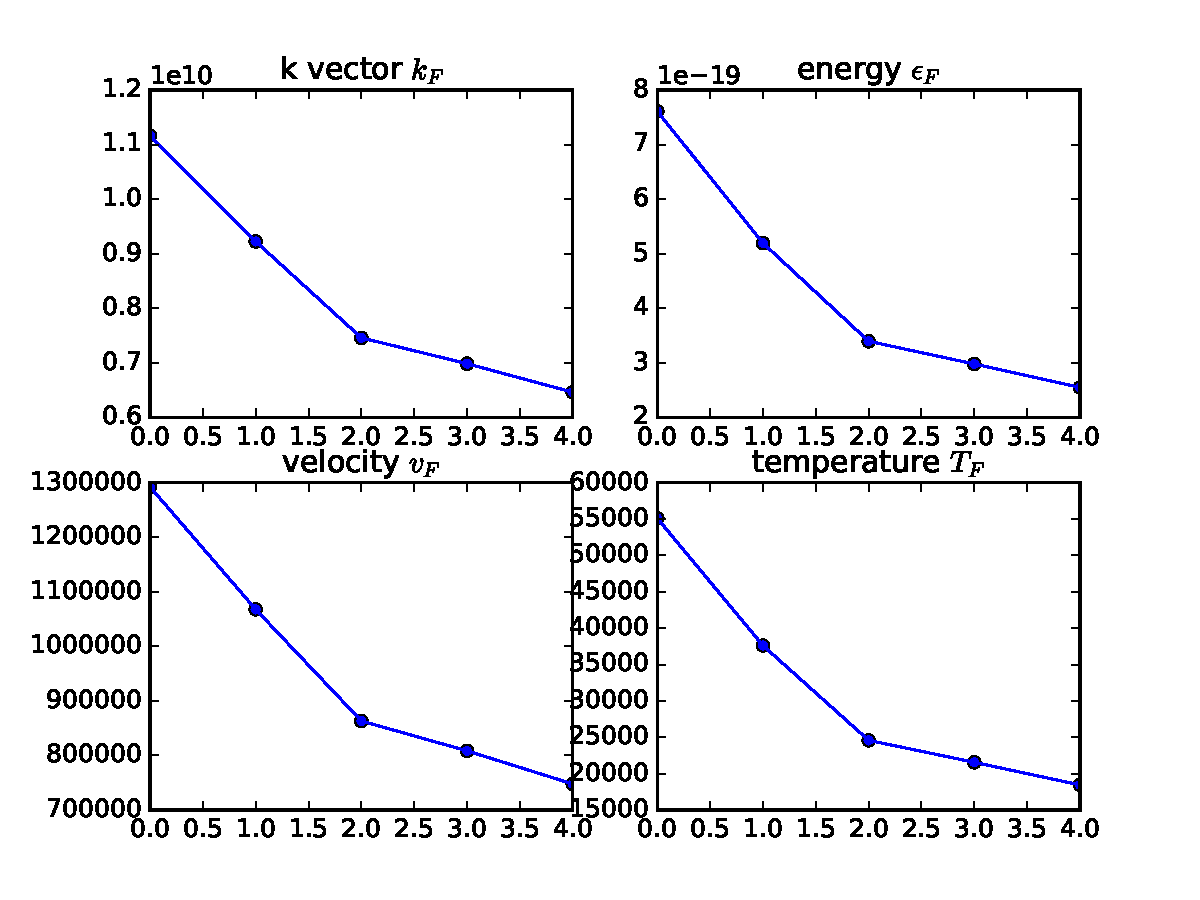
\includegraphics[width = 0.7\linewidth]{4plot.pdf}
	\centering
	\caption{Four plots showing the trends for fermi energy, wavevector, velocity and temperature for the alkali metals}
\end{figure}

\newpage
\section*{3. Temperature dependence of energy and chemical potential for the Fermi-Dirac distribution}
\subsection*{a)}
At zero temperature we have the following expression for Gibbs energy
\begin{equation*}
	G_{T=0}=N\mu=E+pV
\end{equation*}
In the calculations we need to use the expression for the energy
\begin{equation}
	E(N) = \frac{\hbar^2}{2m_e}\qty(\frac{3\pi^2N}{V})^{2/3}
\end{equation}
We want to insert the pressure and we can get this by volume derivating the energy.
\begin{align*}
	p &= -\qty(\pdv{\epsilon(N)}{V})\\
	&=-\pdv{}{V}\qty( \frac{\hbar^2}{2m_e}\qty(\frac{3\pi^2N}{V})^{2/3}  )\\
	&= \frac{\hbar^2}{2m_e}(3\pi^2N)^{2/3} \tfrac{2}{3}V^{-5/3}
\end{align*}
Skipping a few steps of algebra we see that this term looks very similar to the energy and we can abbreviate a lot by introducing this back in. The Gibbs energy becomes
\begin{equation*}
	G = E + \tfrac{2}{3}E = \tfrac{2}{5}E
\end{equation*}

Now we want an expression for the chemical potential where we can insert the result
\begin{align*}
	\mu = \frac{1}{N}(E+pV)\\
	\mu = \frac{5}{3}\frac{E}{N}
\end{align*}

The assignment gave another hint as to how to find E; integrating the product of the density of states, fermi dirac distribution and energy. 
\begin{align*}
	E = \int_0^\infty DOS\cdot FDD\cdot \epsilon \\
	E = \frac{V}{2\pi^2}\qty(\frac{2m_e}{\hbar^2})^{3/2}\frac{2}{5}\epsilon_F^{5/2}
\end{align*}
If we insert this back into the expression for the chemical potential we see that almost everything cancels out and we are left with
\begin{equation}
	\mu = \epsilon_F
\end{equation}

\newpage
\subsection*{b)}

With unitless variables this is what the fermi dirac distribution looks like. It does not match completely but is good approximation.

\begin{figure}[H]
	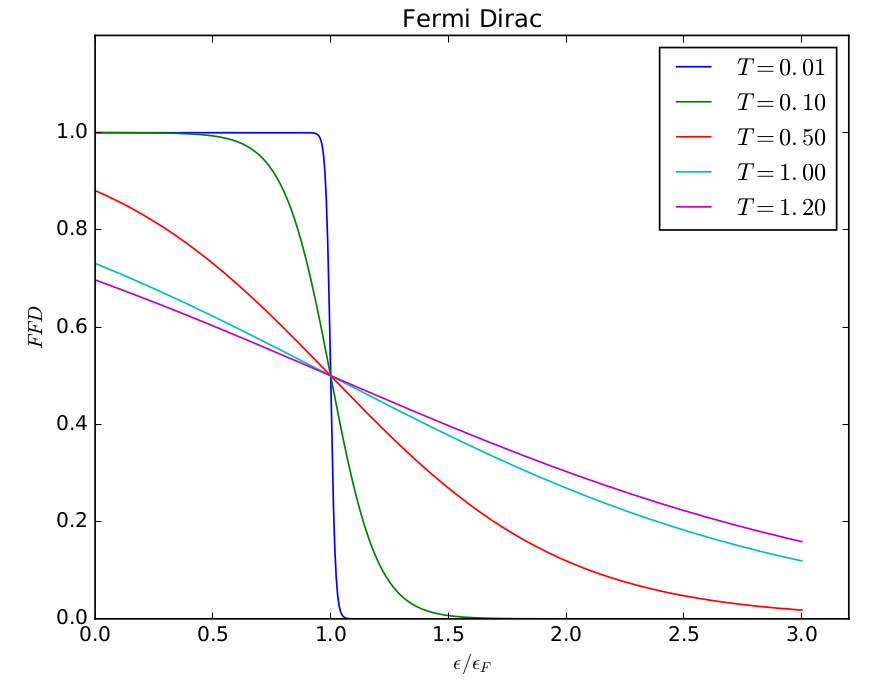
\includegraphics[width = 0.7\linewidth]{fdd.png}
	\centering
	\caption{The fermi dirac distribution for various temperatures}
\end{figure}

\newpage
\section*{4. DOS in 1D \& 2D FEFG}

\subsection*{a)}
\begin{align*}
	DOS_{2D}(E)dE = DOS_{2D}(k)dk\\
	DOS_{2D}(E) = \frac{DOS_{2D}(k)}{\dv{E}{k}}\\
	= \frac{k}{L_z\pi}\frac{2m}{\hbar^2}\frac{1}{2k}
\end{align*}

\subsection*{b)}
\begin{align*}
	DOS_{1D}(E) = \frac{DOS_{1D}(k)}{\dv{E}{k}}\\
	= \frac{1}{\pi}\frac{1}{L_y L_z}\frac{2m}{\hbar^2}\frac{1}{2k}\\
	= \frac{m}{\hbar^2\pi}\frac{1}{L_y L_z} \frac{1}{k}\\
	= \qty(\frac{m}{E})^{1/2}\frac{1}{2\pi\hbar}\frac{1}{L_y L_z}
\end{align*}

\subsection*{c)}
A plot of the DOS for 1D, 2D, and 3D is useful when comparing the different situations.
\begin{figure}[H]
	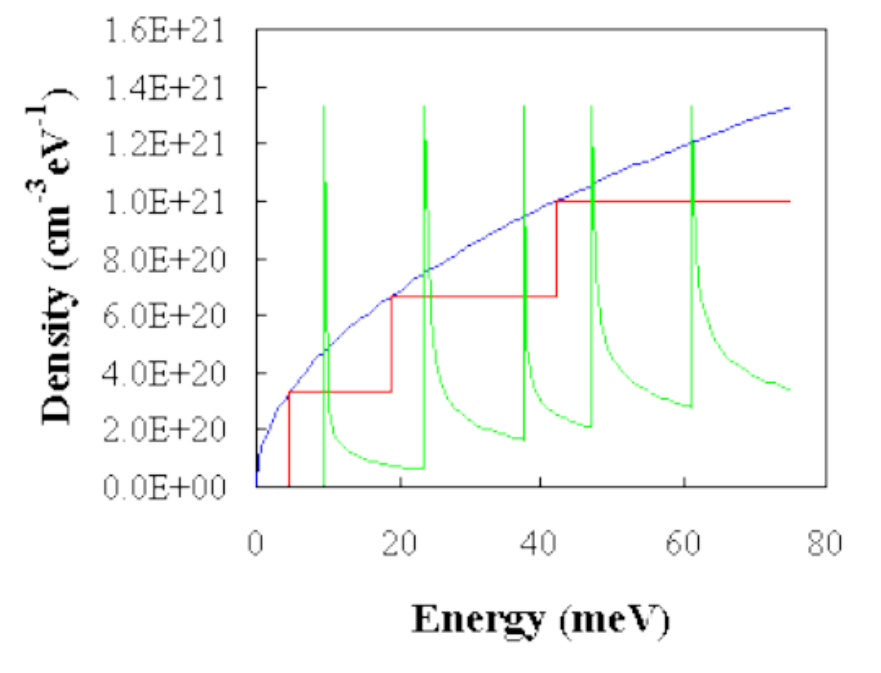
\includegraphics[width = 0.7\linewidth]{dos.png}
	\centering
	\caption{Density of states as function of energy for 1D (green), 2D (red) and 3D (blue)}
\end{figure}

When the dimensionality changes we don't no longer have a uniformity of states distributed in k-space. The blue line in the 3D example illustrates how the number of allowed states pr volume increases when you allow higher and higher energies. This is essentially a sphere that grows in k-space where the sphere radius is the energy. For the 2 dimensional case, however, the states are distributed like planes in k-space, with a big gap between them. Whenever the energy becomes enough to reach the new level the DOS makes a jump before being constant again. It is constant because the introduction of new states is just as rapid as the increase in the spheres volume so that the density remains the same. For the 1D case the available states are are lines in k-space. The geometry of the states' distribution now mean that for each jump in level only some new states are introduced, at a rate slower than the expanding sphere, so the density of states decreses (explicitly with $E^{-1/2}$. That is until the next jump where it follows the same pattern. Quantum wells are analoguous to the 2D example, as we then have constraint in one direction. While quantum wires follows the 1D situaton where the constraint is in two directions.

\subsection*{d)}
The direction of the constraint is arbitrary. It could for example be in the y-direction or the z-direction. But two different configurations of constraint does not change the physics of the system (as the choice of coordinate system is arbitrary). They must therefore lead to the same energy and we get a degeneracy in the states. 

\newpage
\section*{ 6. k-space considerations of some cubic lattices }
\subsection{a)}


\end{document}